\def\languageisenglish{}
\RequirePackage{amsmath}
\documentclass[a4paper,10pt]{extarticle} % extarticle allows to use font size of 8pt.

\usepackage[a4paper, top=2cm, bottom=2cm, left=2cm, right=2cm]{geometry} % Marge reduction.

%% Font and typing packages
\usepackage{fontspec}
\setmainfont[
	Ligatures=TeX,
	]{Caladea} % default is Latin Modern
\newfontfamily\titlefont[Ligatures=TeX]{Georgia} % font for front page title
\usepackage{microtype}			% Greatly improves general appearance of the text.
\usepackage{siunitx}			% Unit appearance.
\sisetup{detect-all}				% Avoid using math font in a normal text.
\usepackage{ulem}				% To cross words out. Use \sout{}.
\usepackage{anyfontsize}  % Disable the warnings when a font size isn't available.
\usepackage{unicode-math} % Math characters are copy pasted correctly
\usepackage{accsupp}				% Allows to automatically replace some characters when copy-pasted

\ifdefined\languageisfrench
	%% Language specific package
	\usepackage[french]{babel}
	\frenchbsetup{StandardLists=true} % Necessary to use enumitem with babel/french.
\fi
\ifdefined\languageisenglish
	%% Language specific package
	\usepackage[super]{nth}
\fi
\ifdefined\languageisitalian
	%% Language specific package
	\usepackage[italian]{babel}
\fi
\ifdefined\languageisspanish
	%% Language specific package
	\usepackage[spanish]{babel}
\fi
\ifdefined\languageispolish
	%% Language specific package
	\usepackage[polish]{babel}
\fi
\ifdefined\languageisrussian
	%% Language specific package
	\usepackage[russian]{babel}
\fi
\ifdefined\languageisgerman
	%% Language specific package
	\usepackage[german]{babel}
	\usepackage[super]{nth}
\fi

%% Array utilities
\usepackage{array}				% Additionnal options for arrays.
\usepackage{colortbl}			% Additionnal options for coloring arrays.
\usepackage[table]{xcolor}		% Auto alternate grey-white rows.
\usepackage{multirow}		% make a row from multiple rows

%% List utilities
\usepackage[inline]{enumitem}   % Display inline lists.
\usepackage{etoolbox}           % General utility. Good for lists for instance.
\usepackage{xparse}             % List utilities.

%% Page utilities
\usepackage{graphicx}        % for the \includegraphics command
\usepackage{parskip} 			% no paragraph indentation and spaces between paragraphs.
\usepackage{multicol}			% Allows to divide a part of the page in multiple columns.
\usepackage{fancyhdr}		% For custom headers and foot texts
\usepackage{titlesec}			% title customization
\pagestyle{fancy}
\usepackage{framed}
\usepackage{csquotes}		% automatic quotation marks adapted of the current language. can be summoned with \enquote{X}
	
%% Others
\usepackage{calc}
\usepackage{epstopdf}         % needed to use the .eps format in LuaTeX
\usepackage{xstring}            % String parsing, cutting, etc.
\definecolor{linkcolour}{RGB}{131,25,139}
\usepackage[unicode, colorlinks=true, linkcolor=linkcolour, urlcolor=linkcolour, bookmarks=false, pdfdisplaydoctitle=true, pdfstartview=FitH, pdfpagelabels=true]{hyperref} % Links in PDF.
\usepackage[ocgcolorlinks]{ocgx2}

\makeatletter

%%% Language specific stuff


\ifdefined\languageisenglish
	\def\languagetag{EN}
\fi
\ifdefined\languageisfrench
	\def\languagetag{FR}
\fi
\ifdefined\languageisitalian
	\def\languagetag{IT}
\fi
\ifdefined\languageisspanish
	\def\languagetag{ES}
\fi
\ifdefined\languageispolish
	\def\languagetag{PL}
\fi
\ifdefined\languageisrussian
	\def\languagetag{RU}
\fi
\ifdefined\languageisgerman
	\def\languagetag{DE}
\fi

\def\pathlanguagespecific{../Language_specific/\languagetag/}

% Command related to automatized alphabetical ordering, language specific

\input{\pathlanguagespecific%
alphabeticalordering.tex}

% Characteristics names and abbreviations, profile associated terms

\input{\pathlanguagespecific%
characteristics.tex}

% Anything related to army books, besides unit entries

\input{\pathlanguagespecific%
armybook.tex}

% Magic stuff, and anything related to Paths.

\input{\pathlanguagespecific%
magic.tex}

% Unit entries

\input{\pathlanguagespecific%
unitentry.tex}

% Titlepages

\input{\pathlanguagespecific%
titlepage.tex}

% Stuff specific to the Rulebook

\input{\pathlanguagespecific%
rulebook.tex}

% Stuff specific to the FAQ

\input{\pathlanguagespecific%
faq.tex}

% Model rules and associated

\input{\pathlanguagespecific%
modelrules.tex}

% Quick Ref Sheet

\input{\pathlanguagespecific%
qrs.tex}

% Model classification (size and type)

\input{\pathlanguagespecific%
modelclassification.tex}

% Terrain

\input{\pathlanguagespecific%
terrain.tex}

% Point labels, range, etc.

\input{\pathlanguagespecific%
miscellanous.tex}

% Special items

\input{\pathlanguagespecific%
specialitems.tex}


%%% Technical commands %%%

% Necessary for language_specific
\newcommand{\ifsubstring}[4]{%
\protected@edef\split@temp{#1}%
\protected@edef\split@tempbis{#2}%
\saveexpandmode%
\expandarg\IfSubStr{\split@temp}{\split@tempbis}{#3}{#4}%
\restoreexpandmode%
}

\newcommand{\isitoneornot}[3]{%
% First step is to remove spaces if there are some
\def\numberwithoutspaces{\expandafter\removespaces\expandafter{#1}}%
% Next step is getting rid of formatting if there are any (bold, color, ...)
\pdfstringdef\cleannumber{\numberwithoutspaces}%
%Defining 1 in \pdfstringdef terms (it will add \376\377\000 before usually - unicode identifier)
\pdfstringdef\numberone{1}%
% Now we can try if it is 1 or not
\ifsubstring{\numberone}{\cleannumber}{#2}{#3}%
}

\newcommand{\isthereaplusornot}[3]{%
\ifsubstring{#1}{+}{#2}{#3}%
}

\def\removespaces#1{\zap@space#1 \@empty}

% Other
\newcommand{\leftspecialbracket}{% angle bracket that get replaced by a < when copy pasted
\BeginAccSupp{method=hex,unicode,ActualText=003C}%
$\langle$%
\EndAccSupp{}%
}

\newcommand{\rightspecialbracket}{% angle bracket that get replaced by a > when copy pasted
\BeginAccSupp{method=hex,unicode,ActualText=003E}%
$\rangle$%
\EndAccSupp{}%
}

\newenvironment{hidewhenprinted}{\begin{ocg}[printocg=never]{HideWhenPrinted}{id1}{1}}{\end{ocg}}

\newcommand{\boosted}[1]{\textbf{\textcolor{blue}{$\{$#1$\}$}}}
\newcommand{\base}[1]{\textcolor{red}{\hspace*{-0.25ex}\leftspecialbracket{}#1\rightspecialbracket{}}}
\newcommand{\specialboosted}[1]{\textbf{\textcolor{olive}{\hspace*{-0.25ex}\leftspecialbracket{}\hspace*{-0.4ex}\leftspecialbracket{}#1\rightspecialbracket{}\hspace*{-0.4ex}\rightspecialbracket{}}}}

\newcommand{\newrule}{\textcolor{green!50!black}}
\newcommand{\removedrule}[1]{\textcolor{green!50!black}{\sout{#1}}}
\newcommand{\rewordedrule}{\textcolor{green!60!black}}
\newcommand{\removedreworded}[1]{\textcolor{green!60!black}{\sout{#1}}}
\newcommand{\starsymbol}{$\star$}
\newcommand{\refsymbol}{$^\star$}

\DeclareSIUnit{\degree}{\SIUnitSymbolDegree}
\DeclareSIUnit{\inch}{″}
\DeclareSIUnit{\foot}{′}
\newcommand{\range}[1] {\labels@range~#1\si{\inch}}
\newcommand{\distance}[1] {#1\si{\inch}}
\newcommand{\result}[1] {‘#1’}

\newcommand{\verysmallfontsize}{\fontsize{4}{4.8}\selectfont}
\newcommand{\smallfontsize}{\fontsize{6}{7.2}\selectfont}
\newcommand{\normalfontsize}{\fontsize{8}{9.6}\selectfont}
\newcommand{\largefontsize}{\fontsize{10}{12}\selectfont}
\newcommand{\largerfontsize}{\fontsize{12}{14.4}\selectfont}
\newcommand{\Largefontsize}{\fontsize{14}{16.8}\selectfont}
\newcommand{\Largerfontsize}{\fontsize{15}{18}\selectfont}
\newcommand{\hugefontsize}{\fontsize{18}{21.6}\selectfont}
\newcommand{\Hugefontsize}{\fontsize{25}{30}\selectfont}

%%% Table of Contents %%%

\newcommand{\toctarget}[1]{%
\phantomsection\label{#1}%
\hypertarget{#1}%
}

\newcommand{\tocentry}[2]{%
\noindent\hyperlink{#1}{#2}\hfill\pageref{#1}%
}


%%% Icons %%%

\newcommand{\alchemyicon}{pics/Icon_alchemy.pdf}
\newcommand{\shamanismicon}{pics/Icon_shamanism.pdf}
\newcommand{\cosmologyicon}{pics/Icon_cosmology.pdf}
\newcommand{\divinationicon}{pics/Icon_divination.pdf}
\newcommand{\druidismicon}{pics/Icon_druidism.pdf}
\newcommand{\evocationicon}{pics/Icon_evocation.pdf}
\newcommand{\occultismicon}{pics/Icon_occultism.pdf}
\newcommand{\pyromancyicon}{pics/Icon_pyromancy.pdf}
\newcommand{\witchcrafticon}{pics/Icon_witchcraft.pdf}
\newcommand{\thaumaturgyicon}{pics/Icon_thaumaturgy.pdf}

\newcommand{\cosmologychaosicon}{pics/Icon_cosmology_chaos.pdf}
\newcommand{\cosmologycosmosicon}{pics/Icon_cosmology_cosmos.pdf}

%%% Headers %%%

\renewcommand{\headrulewidth}{0pt}
% Footers defined in the main .tex file to customize order

\newcommand{\footerlogosize}{0.5cm}

\setlength{\columnsep}{1cm}

%%% Table parameters %%%

\newcolumntype{M}[1]{>{\centering\let\newline\\\arraybackslash\hspace{0pt}}m{#1}}
\newcolumntype{P}[1]{>{\centering\let\newline\\\arraybackslash\hspace{0pt}}p{#1}}

\setlength{\tabcolsep}{0pt}
\renewcommand{\arraystretch}{1.55}

\arrayrulecolor{black!50}
\setlength{\arrayrulewidth}{0.5pt}

\newcommand{\newpathlogo}[2]{\clearpage\begin{center}\toctarget{#2}{\includegraphics[height=1.8cm]{#1}}\end{center}}

\newcommand{\starttable}[2]{%
\begin{center}
\begin{tabular}{m{0.53\linewidth}m{0.47\linewidth}}
\rowcolor[RGB]{#1}\multicolumn{2}{p{\linewidth}}{%
\rule{0pt}{0.7cm}% setting a minimum height
\centering\hugefontsize\textbf{#2}}\tabularnewline%
}

\newcommand{\tablepassive}[2]{%
\multicolumn{2}{p{\linewidth}}{%
\textbf{#1}\spacebeforecolon{}: #2}\tabularnewline
}

\newcommand{\tablelabels}{%
\hspace*{0.08\linewidth}\begin{tabular}{M{0.14\linewidth}M{0.24\linewidth}m{0.25\linewidth}m{0.29\linewidth}}
\textit{\spellsCastingValue}&
\textit{\spellsRange}&
\textit{\spellsType}&
\textit{\spellsDuration}\tabularnewline
\end{tabular}&
\textit{\spellsEffect}\tabularnewline
\hline
}

\newcommand{\spelllabelandtitle}[2]{%
\begin{tabular}{@{}M{0.08\linewidth}@{}m{0.92\linewidth}@{}}%
{\Largefontsize\textbf{#1}}&%
%\makebox[0.08\linewidth]{\Largefontsize\textbf{#1}}
{\Largefontsize\textbf{#2}}\tabularnewline%
\end{tabular}%
}

\newcommand{\replabel}{\newline\textit{\largefontsize\replicablespellnumber}}

\newcommand{\tablespellcastingvalue}[1]{%
\vspace*{-5pt}
\hspace*{0.08\linewidth}\begin{tabular}{M{0.14\linewidth}M{0.24\linewidth}m{0.25\linewidth}m{0.29\linewidth}}
\textbf{#1}&
}

\newcommand{\tablespellrange}[1]{%
\textbf{#1}&
}

\newcommand{\tablespelltype}[1]{%
#1 &
}

\newcommand{\tablespellduration}[1]{%
#1\tabularnewline
\end{tabular}
&
}

\newcommand{\tablespelleffect}[1]{%
#1\tabularnewline
}

\newcommand{\closetable}{%
\end{tabular}
\end{center}
}

\newcommand{\newcosmologylogo}{\clearpage\begin{center}\toctarget{cosmology}{\hspace*{0.3cm}\includegraphics[width=0.5cm]{\cosmologycosmosicon}\hspace*{4.35cm}\includegraphics[height=1.8cm]{\cosmologyicon}\hspace*{3.95cm}\includegraphics[width=0.8cm]{\cosmologychaosicon}}\end{center}}

\newcommand{\starttablecosmology}{%
\begin{center}%
\begin{tabular}{M{0.05\linewidth}m{0.15\linewidth}M{0.18\linewidth}m{0.12\linewidth}M{0.15\linewidth}M{0.1\linewidth}m{0.25\linewidth}}%
\rowcolor[RGB]{\colors@cosmology}\multicolumn{7}{p{\linewidth}}{%
\rule{0pt}{0.7cm}% setting a minimum height
\centering{%
\begin{minipage}{\widthof{\textbf{\cosmos}}}\vspace*{-0.35cm}\textbf{\textcolor{white}{\cosmos}}\end{minipage}%
\hspace*{3.5cm}%
\begin{minipage}{\widthof{\hugefontsize\textbf{\cosmology}}}{\vspace*{-0.2cm}\hugefontsize\textbf{\textcolor{white}{\cosmology}}}\end{minipage}%
\hspace*{3.5cm}%
\begin{minipage}{\widthof{\textbf{\chaos}}}\vspace*{-0.35cm}\textbf{\textcolor{white}{\chaos}}\end{minipage}%
}}\tabularnewline%
}

\newcommand{\tablepassivecosmology}[2]{%
\multicolumn{7}{p{\linewidth}}{%
\textbf{#1}\spacebeforecolon{}: #2}\tabularnewline
}

\newcommand{\tablelabelscosmology}{%
\hline
&\textit{\spellsType}&
\textit{\spellsDuration}&&
\textit{\spellsCastingValue}&
\textit{\spellsRange}&
\tabularnewline
\hline
}

\newcommand{\spelllabelandtitlecosmology}[2]{%
\Largefontsize\textbf{#1}&
\multicolumn{3}{m{0.45\linewidth}}{\Largefontsize\textbf{#2}}&
}

\newcommand{\tablespellcastingvaluecosmology}[1]{%
\textbf{#1}&
}

\newcommand{\tablespellrangecosmology}[1]{%
\textbf{#1}&\tabularnewline
}

\newcommand{\tablecosmosicon}{\vspace*{-0.15cm}\includegraphics[width=0.4cm]{\cosmologycosmosicon}&}
\newcommand{\tablechaosicon}{\vspace*{0.05cm}\includegraphics[width=0.5cm]{\cosmologychaosicon}&}

\newcommand{\tablespelltextcosmology}[1]{\multicolumn{4}{m{0.62\linewidth}}{#1}\tabularnewline}




\def\colors@alchemy{255,215,0}
\def\colors@shamanism{114,56,16}
\def\colors@cosmology{0,57,116}
\def\colors@divination{47,191,226}
\def\colors@druidism{127,223,90}
\def\colors@evocation{94,29,101}
\def\colors@occultism{222,0,100}
\def\colors@pyromancy{204,0,0}
\def\colors@witchcraft{135,139,166}
\def\colors@thaumaturgy{0,84,34}


% SPELL FORMAT FOR CONSISTENCY

% #1 : Spell name
% #2 : Spell path
\newcommand{\spellformat}[2]{\textit{#1}\ifblank{#2}{}{ (#2)}}


% Titles

\titleformat{\paragraph}{\normalfont\normalsize\bfseries}{\theparagraph}{1em}{}
\titlespacing*{\paragraph}{0pt}{2.5ex plus 1ex minus .2ex}{0.5ex plus .2ex}

\newcommand{\basictitle}[2]{%
\section*{}\vspace*{-20pt}\noindent\begin{center}\toctarget{#1}{\Largerfontsize\textbf{#2}}\end{center}\vspace*{10pt}
}

\newcommand{\basicsubtitle}[1]{%
\noindent{\largerfontsize\textbf{#1}}
}

\newcommand{\basicsubsubtitle}[1]{%
\noindent{\largefontsize\textbf{#1}}
}


\newcommand{\booktitle}{Paths of Magic}
\newcommand{\preversion}{\nth{2} Edition, beta version }
\newcommand{\version}{0.204.1}
%\newcommand{\releasedate}{April 1, 2022} % uncomment if you want to set the date yourself, else it will be today's date
%\newcommand{\translationversion}{PROOFREADING VERSION} % If you want to add a note below the version, for example a translation version

\hypersetup{pdftitle={T9A - \booktitle{} - \version}}

% Footer, you may change the order to follow the alphabetical order of your language

\fancyfoot[L]{\strut\begin{hidewhenprinted}%
\normalfontsize
\hyperlink{tableofcontents}{\tableofcontentsInitials}\hspace*{1cm}
\hyperlink{alchemy}{\includegraphics[height=\footerlogosize]{\alchemyicon}}\hspace*{0.3cm}
\hyperlink{cosmology}{\includegraphics[height=\footerlogosize]{\cosmologyicon}}\hspace*{0.3cm}
\hyperlink{divination}{\includegraphics[height=\footerlogosize]{\divinationicon}}\hspace*{0.3cm}
\hyperlink{druidism}{\includegraphics[height=\footerlogosize]{\druidismicon}}\hspace*{0.3cm}
\hyperlink{evocation}{\includegraphics[height=\footerlogosize]{\evocationicon}}
\end{hidewhenprinted}}
\fancyfoot[R]{\strut\begin{hidewhenprinted}%
\normalfontsize
\hyperlink{occultism}{\includegraphics[height=\footerlogosize]{\occultismicon}}\hspace*{0.3cm}
\hyperlink{pyromancy}{\includegraphics[height=\footerlogosize]{\pyromancyicon}}\hspace*{0.3cm}
\hyperlink{shamanism}{\includegraphics[height=\footerlogosize]{\shamanismicon}}\hspace*{0.3cm}
\hyperlink{thaumaturgy}{\includegraphics[height=\footerlogosize]{\thaumaturgyicon}}\hspace*{0.3cm}
\hyperlink{witchcraft}{\includegraphics[height=\footerlogosize]{\witchcrafticon}}\hspace*{1cm}
\hyperlink{magicphasesummary}{\summariesInitials}
\end{hidewhenprinted}}

% Document Titles

\newcommand{\howtousethisdoc}{How to Use this Document}
\newcommand{\magicphasesummary}{Magic Phase Summary}

% Paths Table of Contents names

\newcommand{\alchemyTOC}{Alchemy}
\newcommand{\shamanismTOC}{Shamanism}
\newcommand{\cosmologyTOC}{Cosmology}
\newcommand{\divinationTOC}{Divination}
\newcommand{\druidismTOC}{Druidism}
\newcommand{\evocationTOC}{Evocation}
\newcommand{\occultismTOC}{Occultism}
\newcommand{\pyromancyTOC}{Pyromancy}
\newcommand{\witchcraftTOC}{Witchcraft}
\newcommand{\thaumaturgyTOC}{Thaumaturgy}

% Titlepage, you may change the order to follow the alphabetical order of your language

\newcommand{\titlepagelefticons}{%
\includegraphics[height=\iconheight]{\alchemyicon}

\vspace*{\spacebetweeniconrows}

\includegraphics[height=\iconheight]{\divinationicon}

\vspace*{\spacebetweeniconrows}

\includegraphics[height=\iconheight]{\evocationicon}

\vspace*{\spacebetweeniconrows}

\includegraphics[height=\iconheight]{\pyromancyicon}

\vspace*{\spacebetweeniconrows}

\includegraphics[height=\iconheight]{\thaumaturgyicon}
}

\newcommand{\titlepagetoc}{%
\tocentry{alchemy}{\alchemyTOC}

\tocentry{cosmology}{\cosmologyTOC}

\tocentry{divination}{\divinationTOC}

\tocentry{druidism}{\druidismTOC}

\tocentry{evocation}{\evocationTOC}

\tocentry{occultism}{\occultismTOC}

\tocentry{pyromancy}{\pyromancyTOC}

\tocentry{shamanism}{\shamanismTOC}

\tocentry{thaumaturgy}{\thaumaturgyTOC}

\tocentry{witchcraft}{\witchcraftTOC}
}

\newcommand{\titlepagerighticons}{%
\includegraphics[height=\iconheight]{\cosmologyicon}

\vspace*{\spacebetweeniconrows}

\includegraphics[height=\iconheight]{\druidismicon}

\vspace*{\spacebetweeniconrows}

\includegraphics[height=\iconheight]{\occultismicon}

\vspace*{\spacebetweeniconrows}

\includegraphics[height=\iconheight]{\shamanismicon}

\vspace*{\spacebetweeniconrows}

\includegraphics[height=\iconheight]{\witchcrafticon}
}

\def\thereisachangelog{} % comment if there is no change log, it will remove the changelog entry in the ToC

% Footers name for ToC and Summaries

\newcommand{\tableofcontentsInitials}{Contents}
\newcommand{\summariesInitials}{Summary}

\newcommand{\characteronly}{Character only}







\begin{document}


\begin{titlepage}
\begin{center}

\ifdef{\booktitle}{}{\newcommand{\booktitle}{Missing title}}
\ifdef{\version}{}{\newcommand{\version}{Missing version}}

{\titlefont\fontsize{40}{48}\selectfont\noindent\theninthage

\fantasybattles}

\vspace*{10pt}

{\titlefont\fontsize{50}{60}\selectfont \booktitle
\vspace{0.4cm}

\fontsize{14}{16.8}\selectfont \ifdef{\preversion}{\preversion}{}\version{}

\ifdef{\releasedate}{\releasedate}{\today}

\ifdef{\translationversion}{{\fontsize{14}{16.8}\selectfont \vspace{3pt}\noindent{}\translationversion}}{}}

\vspace*{20pt}

\newcommand{\iconheight}{1.6cm}
\newcommand{\minipagewidth}{3cm}
\newcommand{\spacebetweeniconrows}{0.8cm}

\hspace*{0.5cm}\begin{minipage}[c]{\minipagewidth}
\begin{center}
\titlepagelefticons

\end{center}
\end{minipage}
\hfill\begin{minipage}[c]{8cm}

{\fontsize{12}{14.4}\selectfont

\hfill\textcolor{white}{\verysmallfontsize d}% debug, else everything goes wild with alignment.
\begin{center}
\hypertarget{tableofcontents}{\tocentry{howtousethisdoc}{\howtousethisdoc}}

\vspace*{5pt}

\titlepagetoc

\vspace*{5pt}

\tocentry{magicphasesummary}{\magicphasesummary}

\ifdef\thereisachangelog{\tocentry{pathschangelog}{\changelog}}{}
\end{center}
}

\end{minipage}\hfill
\begin{minipage}[c]{\minipagewidth}
\begin{center}

\titlepagerighticons{}
\end{center}
\end{minipage}\hspace*{0.5cm}

\vfill

\begin{tabular}{@{}m{2cm}@{\hskip 20pt}m{13cm}@{}}
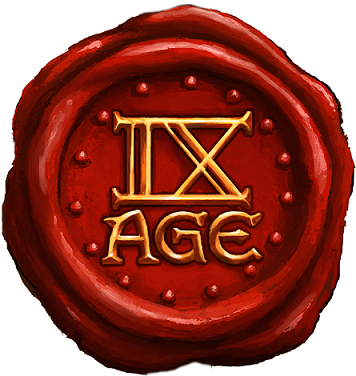
\includegraphics[width=2cm]{../Layout/pics/seal_9th.png} &
{\fontsize{10}{12}\selectfont \textcolor{black!50}{\noindent\frontpagecreditswithoutblue}}

\vspace*{10pt}
\noindent{\fontsize{10}{12}\selectfont \textcolor{black!50}{\license}}
\tabularnewline
\end{tabular}


\end{center}
\end{titlepage}

\setcounter{page}{2}


\basictitle{howtousethisdoc}{\howtousethisdoc}

This document describes the different Paths of Magic available for \nameofthegame{} and as such is to be used in conjunction with the main Rulebook. For convenience, we repeated below the main rules related to spells from the Rulebook, along with the information needed to read the Paths.

\vspace*{5pt}
\basicsubtitle{Spell Classification}

\begin{multicols}{2}

\begin{center}
\basicsubsubtitle{1 to 6 - \learnedspells}
\end{center}

All spells labelled by a number are Learned Spells. They are the main spells of a Path, usually numbered from 1 to 6 (0 to 6 for Druidism). Their assigned number is relevant for the Spell Selection rules (see below).

The player may attempt to cast each \learnedspell{} only once per Magic Phase, even if it is known by different Wizards (unless the spell is Replicable, see below).

\begin{center}
\basicsubsubtitle{\hereditaryspellnumber{} - \hereditaryspells}
\end{center}

Most Army Books contain a \hereditaryspell{} labelled \enquote{\hereditaryspellnumber}. \hereditaryspells{} follow all the rules for \learnedspells{}. Note that this document does not contain any \hereditaryspells{}.

\vspace*{\fill}
\columnbreak

\begin{center}
\basicsubsubtitle{\attributespellnumber{} - \attributespells}
\end{center}

\attributespells{} are labelled \enquote{\attributespellnumber{}}. \wizards{} that know at least one spell from a Path automatically know the Path \attributespell{} (if there is any).

Path \attributespells{} cannot be cast independently. Instead, the Caster may cast the \attributespell{} automatically whenever it successfully casts a \learnedspell{} from the same Path. \attributespells{} cannot be dispelled.

\begin{center}
\basicsubsubtitle{\textit{\replicablespellnumber} - \replicablespells}
\end{center}

Additionally, some Learned Spells are Replicable Spells. These are labelled \enquote{\replicablespellnumber}. The player may attempt to cast \replicablespells{} multiple times in the same magic phase. Each Wizard may only make a single attempt, however.

\vspace*{\fill}
\end{multicols}
\vspace*{-10pt}

\basicsubtitle{Spell Selection}

\begin{itemize}[label={-}]
\item \textbf{\wizardapprentices} know \textbf{1 spell} selected between \textbf{1} and \textbf{\hereditaryspellnumber}.
\item \textbf{\wizardadepts} know \textbf{2 spells} selected from \textbf{1}, \textbf{2}, \textbf{3}, \textbf{4} and \textbf{\hereditaryspellnumber}.
\item \textbf{\wizardmasters} know \textbf{4 spells} selected from \textbf{1}, \textbf{2}, \textbf{3}, \textbf{4}, \textbf{5}, \textbf{6} and \textbf{\hereditaryspellnumber}.
\end{itemize}

\vspace*{5pt}
\basicsubtitle{Spell Properties}

\begin{multicols}{3}\raggedcolumns

\begin{center}
\basicsubsubtitle{Spell Name}

Use the spell name to state which spell you intend to cast.

\basicsubsubtitle{\spellsEffect}

The effect of a spell defines what happens to the target of the spell when the spell is successfully cast. Spell effects are never affected by Special Equipment, Model Rules, other spell effects or similar abilities affecting the Caster, unless noted otherwise.
\end{center}

\vspace*{\fill}\columnbreak

\begin{center}
\basicsubsubtitle{\spellsType}

It describes how the spell's targets can be chosen. A spell can have more than one type. Unless stated otherwise, a spell may only have a single target and the target must be a single unit. If a spell has more than one type, apply all the restrictions.

\basicsubsubtitle{\spellsDuration}

It determines how long the effects of the spell are applied.
\end{center}
\vspace*{\fill}\columnbreak

\begin{center}
\basicsubsubtitle{\spellsCastingValue}

It is the minimum value you need to reach to succeed a Casting Attempt. Spells may have different Casting Values available (see Boosted Spells).

\basicsubsubtitle{\spellsRange}

It determines the maximum distance between the Caster and the target.
\end{center}
\vspace*{\fill}
\end{multicols}

\basicsubtitle{Boosted Spells}

Some spells have two Casting Values, the higher Casting Value being called the Boosted version of the spell. Boosted versions may have their type (range, target restrictions) modified (e.g. giving the spell a longer range), and/or the effects of the spell changed. Declare if you are trying to cast the Boosted version of a spell before rolling any dice. If no declaration is made, the basic version for the chosen target is assumed to be used.

The differences between the spell versions are signified by using the following colour coding: \base{non-Boosted version}, \boosted{Boosted version}, and, in some rare cases, \specialboosted{amplified version}.









% Now the paths. You can copy paste the different paths to follow your alphabetical order



\newpathlogo{\alchemyicon}{alchemy}

\starttable{\colors@alchemy}{\alchemy}

\tablelabels

\spelllabelandtitle{\attributespellnumber}{\alchemyattribute}

\tablespellcastingvalue{}
\tablespellrange{\distance{18}}
\tablespelltype{\hex}
\tablespellduration{\lastsoneturn}
\tablespelleffect{%
The target gains \flammable{} against Melee Attacks.
}
\hline
\spelllabelandtitle{1}{\alchemyspellone}

\tablespellcastingvalue{7+}
\tablespellrange{\distance{24}}
\tablespelltype{\hex\newline\missile\newline\damage}
\tablespellduration{\instant}
\tablespelleffect{%
The target suffers D3+1 hits with \flamingattacks{}, \magicalattacks{}, and Armour Penetration 10. These hits \textbf{always} wound on a roll equal to or greater than 7 - the target's Armour. An unmodified \result{6} always wounds and an unmodified \result{1} always fails to wound. 
}
\hline
\spelllabelandtitle{2}{\alchemyspelltwo}

\tablespellcastingvalue{\base{5+}\newline\boosted{9+}}
\tablespellrange{\distance{24}}
\tablespelltype{\augment}
\tablespellduration{\lastsoneturn}
\tablespelleffect{%
The target gains \base{+1} \boosted{+2} Armour.

}
\hline
\spelllabelandtitle{3}{\alchemyspellthree}

\tablespellcastingvalue{8+}
\tablespellrange{\distance{18}}
\tablespelltype{\augment}
\tablespellduration{\lastsoneturn}
\tablespelleffect{%
The target gains +1 Armour Penetration, \flamingattacks{}, and \magicalattacks{}.
}
\hline
\spelllabelandtitle{4}{\alchemyspellfour}

\tablespellcastingvalue{7+}
\tablespellrange{\distance{24}}
\tablespelltype{\hex\newline\missile\newline\damage}
\tablespellduration{\instant}
\tablespelleffect{%
The target suffers  D3+3 hits with Strength X, Armour Penetration 4, \flamingattacks{}, and \magicalattacks{}, where X is equal to the target's Armour.
}
\hline
\spelllabelandtitle{5}{\alchemyspellfive}

\tablespellcastingvalue{8+}
\tablespellrange{\distance{36}}
\tablespelltype{\hex}
\tablespellduration{\permanent}
\tablespelleffect{%
The target suffers -1 Armour.
}
\hline
\spelllabelandtitle{6}{\alchemyspellsix}

\tablespellcastingvalue{\base{6+}\newline\boosted{9+}}
\tablespellrange{\base{\distance{18}}\newline\boosted{\distance{36}}}
\tablespelltype{\hex\newline\missile\newline\damage}
\tablespellduration{\instant}
\tablespelleffect{%
The target suffers 1 hit with Strength 3 [6], Armour Penetration 10, \magicalattacks{}, \multiplewounds{D3}{}, and \penetrating{}.
}

\closetable{}





\newcosmologylogo

\starttablecosmology

\tablepassivecosmology{\cosmologypassive}{All \cosmology{} spells are divided into two versions, representing opposing aspects; \textbf{\cosmos} and \textbf{\chaos}. When casting \cosmology{} spells, always declare which version of the spell you are using. Whenever the Caster successfully casts a non-Bound Cosmology spell, the next Cosmology spell it attempts to cast has its Casting Value reduced by 1, provided this spell is a Cosmology spell of the opposing aspect.}

\tablelabelscosmology

\spelllabelandtitlecosmology{1}{\cosmologyspellone}
\tablespellcastingvaluecosmology{6+}
\tablespellrangecosmology{\distance{24}}
\tablecosmosicon{}
\textbf{\augment}&
\multirow{2}{*}{\vspace*{-0.3cm}\lastsoneturn}&
\tablespelltextcosmology{The target gains \textbf{+1} Offensive Skill and \textbf{+1} Defensive Skill, and has its weapons' Aim \textbf{improved} by 1.}
\tablechaosicon{}
\textbf{\hex}&
&
\tablespelltextcosmology{The target suffers \textbf{-1} Offensive Skill and \textbf{-1} Defensive Skill, and has its weapons' Aim \textbf{worsened} by 1.}
\hline

\spelllabelandtitlecosmology{2}{\cosmologyspelltwo}
\tablespellcastingvaluecosmology{5+}
\tablespellrangecosmology{\distance{24}}
\tablecosmosicon{}
\textbf{\augment}&
\multirow{2}{*}{\vspace*{-0.85cm}\lastsoneturn}&
\tablespelltextcosmology{Rolls for Charge Range, Flee Distance, Pursuit Distance, and Overrun Distance of units with at least one model affected by the spell are subject to two instances of \textbf{Maximised} Roll.}
\tablechaosicon{}
\textbf{\hex}&
&
\tablespelltextcosmology{Rolls for Charge Range, Flee Distance, Pursuit Distance, and Overrun Distance of units with at least one model affected by the spell are subject to two instances of \textbf{Minimised} Roll.}
\hline

\spelllabelandtitlecosmology{3}{\cosmologyspellthree}
\tablespellcastingvaluecosmology{7+}
\tablespellrangecosmology{\distance{24}}
\tablecosmosicon{}
\multirow{2}{2.5cm}{\vspace*{0cm}\newline\hex{},\newline\missile{},\newline\damage}&
\multirow{2}{*}{\vspace*{-0.8cm}\instant}&
\tablespelltextcosmology{The target suffers 2D6 hits with Strength 4, Armour Penetration 0, and \textbf{\magicalattacks}. Successful \textbf{Special Saves} against wounds caused by this spell must be rerolled.}
\tablechaosicon{}
&
&
\tablespelltextcosmology{The target suffers 2D6 hits with Strength 4 and Armour Penetration 0. Successful \textbf{Armour Saves} against wounds caused by this spell must be rerolled.}
\hline

\spelllabelandtitlecosmology{4}{\cosmologyspellfour}
\tablespellcastingvaluecosmology{8+}
\tablespellrangecosmology{\distance{24}}
\tablecosmosicon{}
\textbf{\augment}&
\multirow{2}{*}{\vspace*{-0.1cm}\lastsoneturn}&
\tablespelltextcosmology{The target gains \textbf{+1} Strength and \textbf{+1} Armour Penetration.}
\tablechaosicon{}
\textbf{\hex}&
&
\tablespelltextcosmology{The target suffers \textbf{-1} Strength and \textbf{-1} Armour Penetration.}
\hline

\spelllabelandtitlecosmology{5}{\cosmologyspellfive}
\tablespellcastingvaluecosmology{11+}
\tablespellrangecosmology{\distance{24}}
\tablecosmosicon{}
\textbf{\augment}&
\textbf{\lastsoneturn}&
\tablespelltextcosmology{All models in the target unit \textbf{gain \aegis{5}}.}
\tablechaosicon{}
\textbf{\hex},\newline\textbf{\direct}, \textbf{\damage}&
\textbf{\instant}&
\tablespelltextcosmology{Each model in the target unit \textbf{suffers a hit with Strength 3, Armour Penetration 0, and \magicalattacks}.}
\hline

\spelllabelandtitlecosmology{6}{\cosmologyspellsix}
\tablespellcastingvaluecosmology{7+}
\tablespellrangecosmology{\distance{24}}
\tablecosmosicon{}
\focused{},\newline\textbf{\augment}&
\multirow{2}{*}{\vspace*{-0.4cm}\instant}&
\tablespelltextcosmology{The target \textbf{Recovers} 1 Health Point.}
\tablechaosicon{}
\focused{}, \textbf{\hex},\newline\textbf{\missile},\newline\textbf{\damage}&
&
\tablespelltextcosmology{The target suffers \textbf{1 hit that automatically wounds} with Armour Penetration 10 and Magical Attacks.}

\closetable{}






\newpathlogo{\divinationicon}{divination}

\starttable{\colors@divination}{\textcolor{white}{\divination}}

\tablepassive{\divinationpassive}{Spells from \divination{} gain \distance{+3} range up to a maximum of \distance{+9} for each additional friendly Wizard within \distance{12} of the Caster.}

\hline
\tablelabels

\spelllabelandtitle{\attributespellnumber}{\divinationattribute}

\tablespellcastingvalue{}
\tablespellrange{\distance{12}}
\tablespelltype{\augment}
\tablespellduration{\lastsoneturn}
\tablespelleffect{%
Discipline Tests of units with all models affected by the spell are subject to Minimised Roll.\newline
A unit cannot be affected by this spell more than once per Magic Phase.
}
\hline
\spelllabelandtitle{1}{\divinationspellone}

\tablespellcastingvalue{\base{7+}\newline\boosted{12+}}
\tablespellrange{\base{\distance{18}}\newline\boosted{\distance{6} \aura{}}}
\tablespelltype{\augment}
\tablespellduration{\lastsoneturn}
\tablespelleffect{%
The target gains +2 Offensive Skill, +2 Defensive Skill, and +2 Agility.
}
\hline
\spelllabelandtitle{2}{\divinationspelltwo}

\tablespellcastingvalue{\base{5+}\newline\boosted{9+}}
\tablespellrange{\distance{18}}
\tablespelltype{\hex\newline\missile\newline\damage}
\tablespellduration{\instant}
\tablespelleffect{%
The target suffers \base{D3} \boosted{D6} hits with \magicalattacks{} that wound automatically, with no Special Saves allowed (note that Armour Saves are allowed).
}
\hline
\spelllabelandtitle{3}{\divinationspellthree}

\tablespellcastingvalue{\base{7+}\newline\boosted{12+}}
\tablespellrange{\base{\distance{18}}\newline\boosted{\distance{6} \aura{}}}
\tablespelltype{\augment}
\tablespellduration{\lastsoneturn}
\tablespelleffect{%
The target gains \distracting{} and \hardtarget{}.
}
\hline
\spelllabelandtitle{4}{\divinationspellfour}

\tablespellcastingvalue{\base{8+}\newline\boosted{12+}}
\tablespellrange{\base{\distance{18}}\newline\boosted{\distance{6} \aura{}}}
\tablespelltype{\augment}
\tablespellduration{\lastsoneturn}
\tablespelleffect{%
The target gains \divineattacks{} and must reroll failed to-hit rolls with Melee \base{and Shooting} Attacks.
}
\hline
\spelllabelandtitle{5}{\divinationspellfive}

\tablespellcastingvalue{\base{7+}\newline\boosted{10+}}
\tablespellrange{\distance{18}}
\tablespelltype{\hex\newline\missile\newline\damage}
\tablespellduration{\instant}
\tablespelleffect{%
The target suffers \base{2D6} \boosted{3D6} hits that wound on 4+ with Armour Penetration 1, \divineattacks{}, and \magicalattacks{}.
}
\hline
\spelllabelandtitle{6}{\divinationspellsix}

\tablespellcastingvalue{9+}
\tablespellrange{\distance{18}}
\tablespelltype{\hex}
\tablespellduration{\lastsoneturn}
\tablespelleffect{%
For each Character in the target unit when the spell is cast, the target suffers -1 to Advance Rate, March Rate, Offensive Skill, Defensive Skill, casting rolls, and to-hit rolls with Shooting Attacks.
}

\closetable{}





\newpathlogo{\druidismicon}{druidism}

\starttable{\colors@druidism}{\druidism}

\tablepassive{\druidismpassive}{All Wizards that know at least one \druidism{} spell (excluding Bound Spells) know the \learnedspell{} \textit{\druidismspellzero} in addition to their other spells.}

\hline
\tablelabels

\spelllabelandtitle{\attributespellnumber}{\druidismattribute}

\tablespellcastingvalue{}
\tablespellrange{\distance{12}}
\tablespelltype{\focused\newline\augment}
\tablespellduration{\instant}
\tablespelleffect{%
The target or its unit \base{Recovers} \specialboosted{Raises} 1 Health Point. No single model can Recover (or Raise) more than 1 Health Point per phase from this spell.
}
\hline
\spelllabelandtitle{0\replabel}{\druidismspellzero}

\tablespellcastingvalue{4+}
\tablespellrange{\caster}
\tablespelltype{\newrule{\caster}}
\tablespellduration{\permanent}
\tablespelleffect{%
If the Caster is affected by \textit{\druidismspellzero}, certain spells are cast with an amplified version. Use any text marked with \specialboosted{~} and ignore any \base{red text}. Successfully casting \textit{\druidismspellzero} does not trigger the Attribute Spell.\newline
This spell ends if the Caster attempts to cast \textit{\druidismspellzero} again, or if the opponent removes one dice from their Magic Dice pool at the end of step 3 of any Magic Phase sequence (after Siphon the Veil). 
}
\hline
\spelllabelandtitle{1}{\druidismspellone}

\tablespellcastingvalue{\base{7+}\newline\specialboosted{6+}}
\tablespellrange{\distance{12}}
\tablespelltype{\augment}
\tablespellduration{\lastsoneturn}
\tablespelleffect{%
The Range of this spell can be measured from the Caster or from any \textbf{\water} Terrain Feature on the table.\newline
The target gains \fortitude{} \base{(5+)} \specialboosted{(4+)}.
}
\hline
\spelllabelandtitle{2}{\druidismspelltwo}

\tablespellcastingvalue{\base{6+}\newline\specialboosted{5+}}
\tablespellrange{\distance{18}}
\tablespelltype{\hex\newline\direct\newline\damage}
\tablespellduration{\instant}
\tablespelleffect{%
The Range of this spell can be measured from the Caster or from any \textbf{\cliffs} Terrain Feature on the table.\newline
The target suffers D6 hits with Strength \base{4} \specialboosted{5}, Armour Penetration \base{1} \specialboosted{2}, and \magicalattacks{}.
}
\hline
\spelllabelandtitle{3}{\druidismspellthree}

\tablespellcastingvalue{\base{6+}\newline\specialboosted{5+}}
\tablespellrange{\distance{12}}
\tablespelltype{\hex}
\tablespellduration{\lastsoneturn}
\tablespelleffect{%
The Range of this spell can be measured from the Caster or from any \textbf{\forest} Terrain Feature on the table.\newline
The target suffers \base{-1} \specialboosted{-2} Offensive Skill, \base{-1} \specialboosted{-2} Defensive Skill, and \base{-1} \specialboosted{-2} to hit with Shooting Attacks.
}
\hline
\spelllabelandtitle{4}{\druidismspellfour}

\tablespellcastingvalue{\base{11+}\newline\specialboosted{10+}}
\tablespellrange{\distance{24}}
\tablespelltype{\augment}
\tablespellduration{\instant}
\tablespelleffect{%
This spell has different effects depending on the target:\newline
\textbf{\sizestandard{} \infantry{}/\beast{}$^{1}$}: Raise \base{4} \specialboosted{6} Health Points.\newline
\textbf{\toweringpresence{}$^{2}$}: Raise \base{1} \specialboosted{1} Health Point.\newline
\textbf{Anything else$^{3}$}: Raise \base{2} \specialboosted{3} Health Points.\newline
$^{1}$ More than half of the models in the unit are both \sizestandard{} Size \textbf{and} either \infantry{} or \beast{} Type.\newline
$^{2}$ More than half of the models in the unit have \toweringpresence{}.\newline
$^{3}$ Use this if neither of the above is applicable.
}
\hline
\spelllabelandtitle{5}{\druidismspellfive}

\tablespellcastingvalue{\base{9+}\newline\specialboosted{8+}}
\tablespellrange{\distance{12}}
\tablespelltype{\augment}
\tablespellduration{\lastsoneturn}
\tablespelleffect{%
The Range of this spell can be measured from the Caster or from any \textbf{Hill} Terrain Feature on the table.\newline
The target gains \base{+2} \specialboosted{+3} Resilience.
}
\hline
\spelllabelandtitle{6}{\druidismspellsix}

\tablespellcastingvalue{\base{7+}\newline\specialboosted{6+}}
\tablespellrange{\distance{12}}
\tablespelltype{\augment\newline\specialboosted{\universal}}
\tablespellduration{\lastsoneturn}
\tablespelleffect{%
Place a Forest underneath the target (this can be substituted by placing a marker or the spell card next to the unit). This Forest \textbf{always} extends to the edges of the unit's Boundary Rectangle (even if the unit moves or changes formation). \specialboosted{If the target is a friendly unit, it gains \strider{\forest}.}
}

\closetable{}










\newpathlogo{\evocationicon}{evocation}

\starttable{\colors@evocation}{\textcolor{white}{\evocation}}

\tablelabels

\spelllabelandtitle{\attributespellnumber}{\evocationattribute}

\tablespellcastingvalue{}
\tablespellrange{}
\tablespelltype{}
\tablespellduration{\instant}
\tablespelleffect{%
If your Veil Token pool contains less than 3 Veil Tokens, you gain one Veil Token. No more than 1 Veil Token can be gained from this spell each Phase.
}
\hline
\spelllabelandtitle{1}{\evocationspellone}

\tablespellcastingvalue{\base{5+}\newline\boosted{9+}}
\tablespellrange{\distance{18}}
\tablespelltype{\augment}
\tablespellduration{\lastsoneturn}
\tablespelleffect{%
The target must reroll failed to-wound rolls with its Melee Attacks \boosted{and gains \lethalstrike{}}.
}
\hline
\spelllabelandtitle{2}{\evocationspelltwo}

\tablespellcastingvalue{7+}
\tablespellrange{\distance{24}}
\tablespelltype{\hex}
\tablespellduration{\lastsoneturn}
\tablespelleffect{%
The target suffers -2 Offensive Skill and -2 Defensive Skill. In addition, a unit with at least one model affected by the spell suffers -1 Discipline.
}
\hline
\spelllabelandtitle{3}{\evocationspellthree}

\tablespellcastingvalue{\base{7+}\newline\boosted{10+}}
\tablespellrange{\base{\distance{24}}\newline\boosted{\distance{18}}}
\tablespelltype{\hex\newline\missile\newline\damage}
\tablespellduration{\instant}
\tablespelleffect{%
Choose \base{1} \boosted{up to 3} models in the target unit (which may be Characters or Champions). Each of them suffers 1 hit that wounds automatically with Armour Penetration 10 and \magicalattacks{}.
}
\hline
\spelllabelandtitle{4}{\evocationspellfour}

\tablespellcastingvalue{\base{6+}\newline\boosted{8+}}
\tablespellrange{\base{\distance{12}}\newline\boosted{\distance{18}}}
\tablespelltype{\augment}
\tablespellduration{\lastsoneturn}
\tablespelleffect{%
The target must reroll failed to-hit rolls with its Close Combat \boosted{and Shooting} Attacks.
}
\hline
\spelllabelandtitle{5}{\evocationspellfive}

\tablespellcastingvalue{\base{6+}\newline\boosted{9+}}
\tablespellrange{\base{\distance{12}}\newline\boosted{\distance{24}}}
\tablespelltype{\focused\newline\hex\newline\missile\newline\damage}
\tablespellduration{\instant}
\tablespelleffect{%
The target suffers D3 hits with Strength 10, Armour Penetration 10, and \magicalattacks{}. When rolling to wound with this attack, use the target's Discipline instead of the target's Resilience.
}
\hline
\spelllabelandtitle{6}{\evocationspellsix}

\tablespellcastingvalue{\base{5+}\newline\boosted{10+}}
\tablespellrange{\base{\distance{12}}\newline\boosted{\distance{9} \aura{}}}
\tablespelltype{\augment}
\tablespellduration{\instant}
\tablespelleffect{%
The target may perform a \base{\distance{8}} \boosted{\distance{6}} Magical Move and gains \ghoststep{} during this move.
}

\closetable{}





\newpathlogo{\occultismicon}{occultism}

\starttable{\colors@occultism}{\textcolor{white}{\occultism}}

\tablepassive{\occultismpassive}{When casting a non-Bound Spell from this Path, right after the casting roll, but before any Dispel Attempt, the Active Player may choose to inflict X hits on the Caster's unit or another friendly unengaged unit within \distance{24}. Each unit may only be targeted by this ability once per Magic Phase.\newline
X is equal to the number of Ranks in the targeted unit, down to a minimum of 2, and up to a maximum of 5. These hits wound automatically and no save of any kind is allowed against them. The last model in a unit can never be removed as a casualty using this ability (any wound that would reduce its Health Point pool to 0 is discarded). Units never take Panic Tests for losing Health Points from \occultismpassive{}.\newline
If at least one wound was caused, the spell is cast with the \specialboosted{amplified} version. In that case, use any text marked with \specialboosted{~}.}

\hline
\tablelabels

\spelllabelandtitle{1}{\occultismspellone}

\tablespellcastingvalue{\base{5+}\newline\boosted{6+}}
\tablespellrange{\base{\distance{24}}\newline\boosted{\distance{12} \aura{}}}
\tablespelltype{\base{\hex\newline\direct\newline\damage}\newline\boosted{\universal}}
\tablespellduration{\instant}
\tablespelleffect{%
The target suffers D6 hits with Strength 4, Armour Penetration 1, and \magicalattacks{}.\newline
\boosted{The Caster's unit is unaffected.}\newline
\specialboosted{If one or more unsaved wounds are caused with this spell, the Caster Recovers 1 Health Point.}
}
\hline
\spelllabelandtitle{2}{\occultismspelltwo}

\tablespellcastingvalue{\base{6+}\newline\boosted{9+}}
\tablespellrange{\base{\caster}\newline\boosted{\distance{12}}}
\tablespelltype{\focused\newline\boosted{\augment}}
\tablespellduration{\lastsoneturn}
\tablespelleffect{%
\boosted{This spell may only target Characters, Champions, and single model units.}\newline
The target \specialboosted{and all models in its unit} gain \aegis{6} \textbf{and} \aegis{+1, max 3+}.
}
\hline
\spelllabelandtitle{3}{\occultismspellthree}

\tablespellcastingvalue{7+}
\tablespellrange{\distance{18}}
\tablespelltype{\hex}
\tablespellduration{\permanent}
\tablespelleffect{%
The target suffers -1 Offensive Skill and -1 Defensive Skill.\newline
\specialboosted{The Caster gains +1 Offensive Skill and +1 Defensive Skill.}
}
\hline
\spelllabelandtitle{4}{\occultismspellfour}

\tablespellcastingvalue{\base{5+}\newline\boosted{8+}}
\tablespellrange{\base{\caster}\newline\boosted{\distance{12}}}
\tablespelltype{\focused\newline\boosted{\augment}}
\tablespellduration{\lastsoneturn}
\tablespelleffect{%
The target gains \breathattack{\magicalattacks{}, \toxicattacks}.\newline
\boosted{This spell may only target Characters, Champions, and single model units.}\newline
\specialboosted{If the \breathattack{} is used as a Shooting Attack, its range is increased to \distance{18}.}
}
\hline
\spelllabelandtitle{5}{\occultismspellfive}

\tablespellcastingvalue{8+}
\tablespellrange{\distance{18}}
\tablespelltype{\hex\newline\direct\newline\damage}
\tablespellduration{\instant}
\tablespelleffect{%
The target suffers 1 hit with Strength 10, Armour Penetration 10, \multiplewounds{D3}{}, and \magicalattacks{}.\newline
\specialboosted{If the target is within \distance{12} of the Caster, the spell targets a single Character or Champion joined to the target unit.}
}
\hline
\spelllabelandtitle{6}{\occultismspellsix}

\tablespellcastingvalue{11+}
\tablespellrange{\distance{12}}
\tablespelltype{\hex\newline\direct\newline\damage}
\tablespellduration{\instant}
\tablespelleffect{%
The target suffers 2D6 hits with Strength 5, Armour Penetration 2, and \magicalattacks{}. \specialboosted{The hits gain +1 Strength and +1 Armour Penetration.}
}

\closetable{}








\newpathlogo{\pyromancyicon}{pyromancy}

\starttable{\colors@pyromancy}{\textcolor{white}{\pyromancy}}

\tablelabels

\spelllabelandtitle{\attributespellnumber}{\pyromancyattribute}

\tablespellcastingvalue{}
\tablespellrange{\distance{24}}
\tablespelltype{\hex\newline\missile\newline\damage}
\tablespellduration{\instant}
\tablespelleffect{%
The target suffers D3 hits with Strength 4, Armour Penetration 0, \flamingattacks{}, and \magicalattacks{}.
}
\hline
\spelllabelandtitle{1}{\pyromancyspellone}

\tablespellcastingvalue{4+}
\tablespellrange{\distance{36}}
\tablespelltype{\hex\newline\missile\newline\damage}
\tablespellduration{\instant}
\tablespelleffect{%
The target suffers D6 hits with Strength 4, Armour Penetration 0, \flamingattacks{}, and \magicalattacks{}.
}
\hline
\spelllabelandtitle{2}{\pyromancyspelltwo}

\tablespellcastingvalue{\base{5+}\newline\boosted{8+}}
\tablespellrange{\base{\distance{24}}\newline\boosted{\distance{12}}}
\tablespelltype{\hex}
\tablespellduration{\instant}
\tablespelleffect{%
The target suffers \base{D6} \boosted{2D6} hits with Strength 4, Armour Penetration 0, \flamingattacks{}, and \magicalattacks{}.
}
\hline
\spelllabelandtitle{3}{\pyromancyspellthree}

\tablespellcastingvalue{\base{8+}\newline\boosted{11+}}
\tablespellrange{\base{\distance{18}}\newline\boosted{\distance{6} \aura{}}}
\tablespelltype{\augment}
\tablespellduration{\lastsoneturn}
\tablespelleffect{%
The target's Melee and Shooting Attacks gain a +1 to-wound modifier, \flamingattacks{}, and \magicalattacks{}.
}
\hline
\spelllabelandtitle{4}{\pyromancyspellfour}

\tablespellcastingvalue{\base{7+}\newline\boosted{10+}}
\tablespellrange{\base{\distance{24}}\newline\boosted{\distance{12}}}
\tablespelltype{\hex\newline\missile\newline\damage}
\tablespellduration{\instant}
\tablespelleffect{%
The target suffers \base{2D6} \boosted{3D6} hits with Strength 4, Armour Penetration 0, \flamingattacks{}, and \magicalattacks{}.
}
\hline
\spelllabelandtitle{5}{\pyromancyspellfive}

\tablespellcastingvalue{8+}
\tablespellrange{\distance{24} \aura{}}
\tablespelltype{\hex\newline\damage}
\tablespellduration{\instant}
\tablespelleffect{%
The target suffers D3+1 hits with Strength 4, Armour Penetration 0, \flamingattacks{}, and \magicalattacks{}.
}
\hline
\spelllabelandtitle{6}{\pyromancyspellsix}

\tablespellcastingvalue{10+}
\tablespellrange{\distance{24}}
\tablespelltype{\hex\newline\direct\newline\damage}
\tablespellduration{\instant}
\tablespelleffect{%
Each model in the target unit suffers 1 hit with Strength 3, Armour Penetration 0, \flamingattacks{}, and \magicalattacks{}.
}

\closetable{}






\newpathlogo{\shamanismicon}{shamanism}

\starttable{\colors@shamanism}{\textcolor{white}{\shamanism}}

\tablelabels

\spelllabelandtitle{\attributespellnumber}{\shamanismattribute}

\tablespellcastingvalue{}
\tablespellrange{\caster}
\tablespelltype{}
\tablespellduration{\lastsoneturn}
\tablespelleffect{%
Melee Attacks against the target can \textbf{never} wound on better than 5+.
}
\hline
\spelllabelandtitle{1}{\shamanismspellone}

\tablespellcastingvalue{\base{5+}\newline\boosted{7+}}
\tablespellrange{\distance{18}}
\tablespelltype{\augment}
\tablespellduration{\lastsoneturn}
\tablespelleffect{%
The target gains \base{+1 Strength and +1 Armour Penetration} \boosted{+1 Resilience}.
}
\hline
\spelllabelandtitle{2}{\shamanismspelltwo}

\tablespellcastingvalue{\base{5+}\newline\boosted{8+}}
\tablespellrange{\base{\distance{24}}\newline\boosted{\distance{48}}}
\tablespelltype{\hex\newline\missile\newline\damage}
\tablespellduration{\permanent}
\tablespelleffect{%
Immediately after successfully casting this spell, the target suffers 5D6 hits with Strength 1, Armour Penetration 0, and \magicalattacks{}. If one or more unsaved wounds are caused, the target suffers -1 to hit with its Shooting Attacks. This spell is immediately ended when the target performs an Advance, March, Charge, or Pursuit Move.
}
\hline
\spelllabelandtitle{3}{\shamanismspellthree}

\tablespellcastingvalue{\base{5+}\newline\boosted{8+}}
\tablespellrange{\base{\distance{9}}\newline\boosted{\distance{18}}}
\tablespelltype{\universal}
\tablespellduration{\lastsoneturn}
\tablespelleffect{%
The target gains \frenzy{} and \battlefocus{}.
}
\hline
\spelllabelandtitle{4}{\shamanismspellfour}

\tablespellcastingvalue{\base{6+}\newline\boosted{10+}}
\tablespellrange{\distance{36}}
\tablespelltype{\hex}
\tablespellduration{\lastsoneturn}
\tablespelleffect{%
All units within \base{\distance{6}} \boosted{\distance{12}} of the target when the spell is cast suffer a -1 to-wound modifier on their \base{Shooting} \boosted{Ranged} Attacks \boosted{including \newrule{effects of spells cast while affected by} \spellformat{\shamanismspellfour}{}}. 
}
\hline
\spelllabelandtitle{5}{\shamanismspellfive}

\tablespellcastingvalue{\base{10+}\newline\boosted{12+}}
\tablespellrange{\distance{96}}
\tablespelltype{\ground}
\tablespellduration{\instant}
\tablespelleffect{%
Summon a \totemicbeast{} (profile below). It must be placed within \base{\distance{1}} \boosted{\distance{10}} of the Board Edge.
}
\hline
\spelllabelandtitle{6}{\shamanismspellsix}

\tablespellcastingvalue{\base{8+}\newline\boosted{11+}}
\tablespellrange{\base{\distance{18}}\newline\boosted{\distance{36}}}
\tablespelltype{\hex}
\tablespellduration{\lastsoneturn}
\tablespelleffect{%
The target suffers a -1 to-hit modifier and treats all Terrain (including Open Terrain) as Dangerous Terrain~(2).
}

\closetable{}

\vfill

\newcommand{\totemicbeastname}{\totemicbeast}
\newcommand{\totemicbeastnameaddon}{(for \shamanismspellfive{})}
\newcommand{\totemicbeastoffrules}{\fearless{}, \randommovement{3D6}}% reorder for alpha order in your language


\unitentry{%
	name=\totemicbeastname{},
	speciallogo={Icon_shamanism.pdf},
	unitsize=1,
	size=\heightlarge{},
	type=\beast{},
	basesize=40\timess{}40,
	global@Ad=\XDsix{3},
	global@Ma=,% No MR value for random movers
	global@Di=7,
	globalrules={\randommovement{\XDsix{3}},\fearless{}},
	defense@HP=3,
	defense@Df=3,
	defense@Re=5,
	defense@Arm=0,
	offensename=\totemicbeastname{},
	offense@At=4,
	offense@Of=3,
	offense@St=5,
	offense@AP=2,
	offense@Ag=3,
	offenserules={\breathattack{\St{} 3, \AP{} 0}},
} % END UNIT ENTRY
% Nothing to edit for translation in this file
\vfill


\newpathlogo{\thaumaturgyicon}{thaumaturgy}

\starttable{\colors@thaumaturgy}{\textcolor{white}{\thaumaturgy}}

\tablepassive{\thaumaturgypassive}{When casting non-\boundspells{} from this Path, all Magic Dice that result in \result{1} must be rerolled. Dice causing a Miscast cannot be rerolled. If a Caster Miscasts when casting a spell from this Path, add a +1 Miscast Modifier.}

\hline
\tablelabels

\spelllabelandtitle{1}{\thaumaturgyspellone}

\tablespellcastingvalue{\base{5+}\newline\boosted{8+}}
\tablespellrange{\distance{24}}
\tablespelltype{\hex\newline\missile\newline\damage}
\tablespellduration{\instant}
\tablespelleffect{%
The target suffers \base{D6} \boosted{D6+1} hits with Strength \base{D6} \boosted{D6+1}, Armour Penetration \base{2} \boosted{3}, and \magicalattacks{}.
}
\hline
\spelllabelandtitle{2}{\thaumaturgyspelltwo}

\tablespellcastingvalue{\base{6+}\newline\boosted{9+}}
\tablespellrange{\distance{24}}
\tablespelltype{\hex}
\tablespellduration{\lastsoneturn}
\tablespelleffect{%
\base{Immediately after successfully casting this spell, roll a D6.}\newline%
\boosted{Choose which effect to apply when casting the spell.}\newline%
\begin{itemize}[label={-}]%
\item \base{If 1-3 is rolled,} the target suffers -1 Resilience.%
\item \base{If 4-6 is rolled,} the target suffers -1 Strength and -1 Armour Penetration.%
\end{itemize}%
}
\hline
\spelllabelandtitle{3}{\thaumaturgyspellthree}

\tablespellcastingvalue{\base{8+}\newline\boosted{8+}}
\tablespellrange{\distance{18}}
\tablespelltype{\hex}
\tablespellduration{\lastsoneturn}
\tablespelleffect{%
Units with at least one model affected by the spell cannot benefit from \base{\commandingpresence} \boosted{\rallyaroundtheflag}.
}
\hline
\spelllabelandtitle{4}{\thaumaturgyspellfour}

\tablespellcastingvalue{\base{5+}\newline\boosted{8+}}
\tablespellrange{\base{\caster}\newline\boosted{\distance{24}}}
\tablespelltype{\focused\newline\boosted{\augment}}
\tablespellduration{\lastsoneturn}
\tablespelleffect{%
The target gains \breathattack{Strength D3+2, Armour Penetration 1, \magicalattacks}.\newline
(Roll the D3 immediately after successfully casting this spell.)\newline
\boosted{This spell may only target Characters, Champions, and single model units.}
}
\hline
\spelllabelandtitle{5}{\thaumaturgyspellfive}

\tablespellcastingvalue{12+}
\tablespellrange{\distance{96}}
\tablespelltype{\ground}
\tablespellduration{\permanent}
\tablespelleffect{%
Place a counter on the target point. At the end of each subsequent Magic Phase roll a D6; if 1-3 is rolled, add another counter on the same point. If 4-6 is rolled, each unit within \distance{(2D6+X)}, where X is equal to the number of counters, suffers 2D6 hits with Strength 5, Armour Penetration 2, and \magicalattacks{}. If a unit fails a Panic Test forced by the spell, it flees directly away from the marked point. The spell then ends, remove all counters.
}
\hline
\spelllabelandtitle{6}{\thaumaturgyspellsix}

\tablespellcastingvalue{\base{7+}\newline\boosted{10+}}
\tablespellrange{\base{\distance{12}}\newline\boosted{\distance{18}}}
\tablespelltype{\focused\newline\hex\newline\missile\newline\damage}
\tablespellduration{\instant}
\tablespelleffect{%
The Caster rolls D3+1 and the target rolls D3. If the Caster's roll is higher, the target suffers a number of hits equal to the difference between their respective rolls. These hits wound automatically with Armour Penetration 10 and \magicalattacks{}.
}

\closetable{}







\newpathlogo{\witchcrafticon}{witchcraft}

\starttable{\colors@witchcraft}{\textcolor{white}{\witchcraft}}

\tablelabels

\spelllabelandtitle{\attributespellnumber}{\witchcraftattribute}

\tablespellcastingvalue{}
\tablespellrange{\distance{24}}
\tablespelltype{\universal}
\tablespellduration{\lastsoneturn}
\tablespelleffect{%
If this spell targets a friendly unit, the target gains +1 Advance Rate and +2 March Rate.\newline
If this spell targets an enemy unit, the target suffers -1 Advance Rate and -2 March Rate, to a minimum of 3 and 6 respectively.\newline
A unit cannot be affected by this spell more than twice in the same Magic Phase.
}
\hline
\spelllabelandtitle{1}{\witchcraftspellone}

\tablespellcastingvalue{\base{7+}\newline\boosted{9+}}
\tablespellrange{\distance{24}}
\tablespelltype{\augment}
\tablespellduration{\instant}
\tablespelleffect{%
The target may perform a \base{\distance{8}} \boosted{\distance{12}} Magical Move and gains Fly during this move. Nominate a single model part affected by the spell. This model part may perform a \sweepingattack{} during the move (possibly in addition to other \sweepingattack{}s). This \sweepingattack{} causes D6 hits with Strength 4, Armour Penetration 1, and \magicalattacks{}.
}
\hline
\spelllabelandtitle{2}{\witchcraftspelltwo}

\tablespellcastingvalue{\base{4+}\newline\boosted{7+}}
\tablespellrange{\distance{24}}
\tablespelltype{\hex}
\tablespellduration{\lastsoneturn}
\tablespelleffect{%
The target suffers \base{-1} \boosted{-2} Offensive Skill, \base{-1} \boosted{-2} Defensive Skill, and \base{-1} \boosted{-2} Agility.
}
\hline
\spelllabelandtitle{3}{\witchcraftspellthree}

\tablespellcastingvalue{\base{6+}\newline\boosted{8+}}
\tablespellrange{\distance{36}}
\tablespelltype{\hex}
\tablespellduration{\lastsoneturn}
\tablespelleffect{%
The target cannot use Shooting Attacks \boosted{and suffers a -2 modifier to its casting rolls}.
}
\hline
\spelllabelandtitle{4}{\witchcraftspellfour}

\tablespellcastingvalue{\base{8+}\newline\boosted{10+}}
\tablespellrange{\distance{24}}
\tablespelltype{\hex}
\tablespellduration{\lastsoneturn}
\tablespelleffect{%
Close Combat Attacks made by \boosted{and allocated against} \rnf{} models in the target unit are \textbf{set} to hit and wound on a 4+, regardless of Offensive Skill, Defensive Skill, Strength, and Resilience. Apply this effect before other to-hit and to-wound modifiers.
}
\hline
\spelllabelandtitle{5}{\witchcraftspellfive}

\tablespellcastingvalue{\base{8+}\newline\boosted{8+}}
\tablespellrange{\distance{18}}
\tablespelltype{\universal}
\tablespellduration{\lastsoneturn}
\tablespelleffect{%
The target gains \randommovement{\base{2D6} \boosted{3D6}}.
}
\hline
\spelllabelandtitle{6}{\witchcraftspellsix}

\tablespellcastingvalue{\base{9+}\newline\boosted{11+}}
\tablespellrange{\distance{24}}
\tablespelltype{\hex}
\tablespellduration{\lastsoneturn}
\tablespelleffect{%
Natural to-hit and to-wound rolls of \result{6} of Melee \boosted{and Shooting} Attacks made by the target must be rerolled.
}

\closetable{}







\clearpage
\basictitle{magicphasesummary}{Magic Phase Summary}

{
COMING SOON
%\normalfontsize
%\renewcommand{\arraystretch}{1.5}
%\setlength{\tabcolsep}{6pt}
%\begin{multicols}{2}\raggedcolumns
%
%\paragraph{Magic Phase Sequence}
%
%\begin{tabular}{c|p{6.95cm}}
%1 & Start of the Magic Phase. Roll for the Magic Flux and Channelling. \tabularnewline
%2 & \enquote{\remainsinplay{}} spells may be dispelled. \tabularnewline
%3 & The Active Player may attempt to cast one spell. \tabularnewline
%4 & Repeat steps 2-3 of this Sequence until neither player performed an action. \tabularnewline
%5 & End of the Magic Phase. Resolve end of phase triggered abilities. \tabularnewline
%\end{tabular}
%
%\vspace*{10pt}
%\paragraph{Casting Attempt}
%
%\begin{tabular}{c|m{6.95cm}}
%1 & The Active Player declares a \wizard{}, spell, version of the spell, target of the spell and an amount of Magic Dice (between 1 and 5). \tabularnewline
%2 & The Active Player rolls that many Magic Dice (from the Magic Dice pool). Add the results of the rolled dice and any casting modifiers together to get the total casting roll. \tabularnewline
%3 & The Casting Attempt is successful if the total casting roll is \textbf{equal to or higher} than the spell's Casting Value. Otherwise, the caster suffers from \lostfocus{} and the Casting Attempt failed. \tabularnewline
%\end{tabular}
%
%\vspace*{10pt}
%\paragraph{Dispel Attempt}
%
%\begin{tabular}{c|m{6.95cm}}
%1 & The Reactive Player declares which (if any) of their non-fleeing \wizards{} will attempt to dispel the spell and how many Magic Dice will be used. A minimum of 1 and up to all the dice in your dice pool can be used. A dispel may be attempted even without having any \wizard{}. \tabularnewline
%2 & The Reactive Player rolls that many Magic Dice (from the Magic Dice pool). Add the results of the rolled dice and any dispel modifiers together to get the total dispel roll. \tabularnewline
%3 & The Dispel Attempt is successful if the total dispel roll is \textbf{equal to or higher} than the total casting roll. If so, the spell is dispelled, and the casting failed. Otherwise, the Dispel Attempt fails and the dispeling \wizard{} suffers from \lostfocus{}. \tabularnewline
%\end{tabular}
%
%\vspace*{20pt}
%
%\begin{framed}
%\vspace*{-17pt}
%\paragraph{Magic Modifiers}
%
%\noindent \wizardapprentice{}: +1
%
%\vspace*{3pt}
%\noindent \wizardmaster{}: +2
%
%\vspace*{3pt}
%\noindent The sum of modifiers cannot exceed +3.
%
%\vspace*{3pt}
%\noindent Dispelling \boundspells{}: +1 (may exceed +3)
%
%\end{framed}
%
%\vspace*{\fill}
%\columnbreak
%
%\begin{framed}
%\vspace*{-17pt}
%\paragraph{\overwhelmingpower}
%
%When casting a spell and two or more Magic Dice roll a natural \result{6}, immediately roll one of your unused Magic Dice (if you have any) and add this to the Casting Roll. This may exceed the normal limit of max. 5 Magic Dice to cast spells. If the spell is not dispelled, the casting \wizard{} must roll on the \miscast{} Table.
%
%\end{framed}
%
%\paragraph{\miscast{} Table}
%
%\vspace*{-10pt}
%\renewcommand{\arraystretch}{2}
%\begin{center}
%\begin{tabular}{>{\raggedleft}p{1.7cm}p{5.4cm}}
%\hline
%
%\textbf{\miscast{} Roll:}
%
%(D3+1)$\times$MDU &
%\textbf{\miscast{} effect}
%
%(apply all relevant effects)\tabularnewline
%
%\hline
%
%\textbf{Always} & \textbf{\witchfire}
%
%\vspace*{3pt}
%Caster's unit suffers a number of hits equal to the \miscast{} Roll. The number of hits cannot exceed the total number of Wounds in the unit. These hits have Strength MDU, \magicalattacks{} and \armourpiercing{1}.\tabularnewline
%
%\textbf{10+} & \textbf{\amnesia}
%
%\vspace*{3pt}
%Roll a D6: On 4+,\newline
%the \wizard{} cannot cast the \miscast{} Spell this game anymore.\tabularnewline
%
%\textbf{15+} & \textbf{\catastrophicdetonation}
%
%\vspace*{3pt}
%Roll a D6: On 4+,\newline
%the \wizard{} loses a number of Wounds equal to half its starting number of Wounds, rounding fractions up (no saves of any kind allowed).\tabularnewline
%
%\textbf{20+} & \textbf{\breachintheveil}
%
%\vspace*{3pt}
%Roll a D6: On 4+,\newline
%the \wizard{} is dead, remove it from the game as a casualty (no saves of any kind allowed).\tabularnewline
%\hline
%\end{tabular}
%\end{center}
%\renewcommand{\arraystretch}{1.5}
%
%\vspace*{5pt}
%\noindent Apply all relevant effects.\newline
%\textbf{MDU}: Magic Dice Used, excluding additional dice from \overwhelmingpower{}.
%
%\vspace*{10pt}
%
%\begin{framed}
%\vspace*{-17pt}
%\paragraph{\boundspells{}}
%
%To successfully cast a \boundspell{}, the casting roll must be equal to or higher than the spell's Power Level.
%\begin{itemize}[label={-}]
%\item No positive casting modifiers can be added to the casting roll.
%\item The caster of a \boundspell{} never suffers from \lostfocus{}.
%\item A \boundspell{} does not get the casting modifier from an \overwhelmingpower{}.
%\item Path Attribute is resolved as usual.
%\item Dispelling Attempts gain a +1 modifier, which may exceed the normal limit of max. +3.
%\end{itemize}
%
%If \overwhelmingpower{} is rolled and the spell is not dispelled:\newline
%If MDU is 4 or more, the \boundspell{} is lost and cannot be used again during the game.
%\end{framed}
%
%\vspace*{\fill}
%\end{multicols}
%}

}

\clearpage
\basictitle{pathschangelog}{Change Log}

\vspace*{1cm}
\basicsubtitle{0.204.1}

\begin{itemize}[label={-}]
\item Green text from 0.204.0 removed.
\item Druidism, The Oaken Throne, was missing Type.
\item Occultism, Hand of Glory, was missing Type.
\item Shamanism, \shamanismspellfour{}, clarification of which spells effects are affected.
\end{itemize}

\end{document}

